\subsection{Building a mesh}

\begin{frame}
    \frametitle{Examples}

    \begin{figure}[!ht]
        \centering
        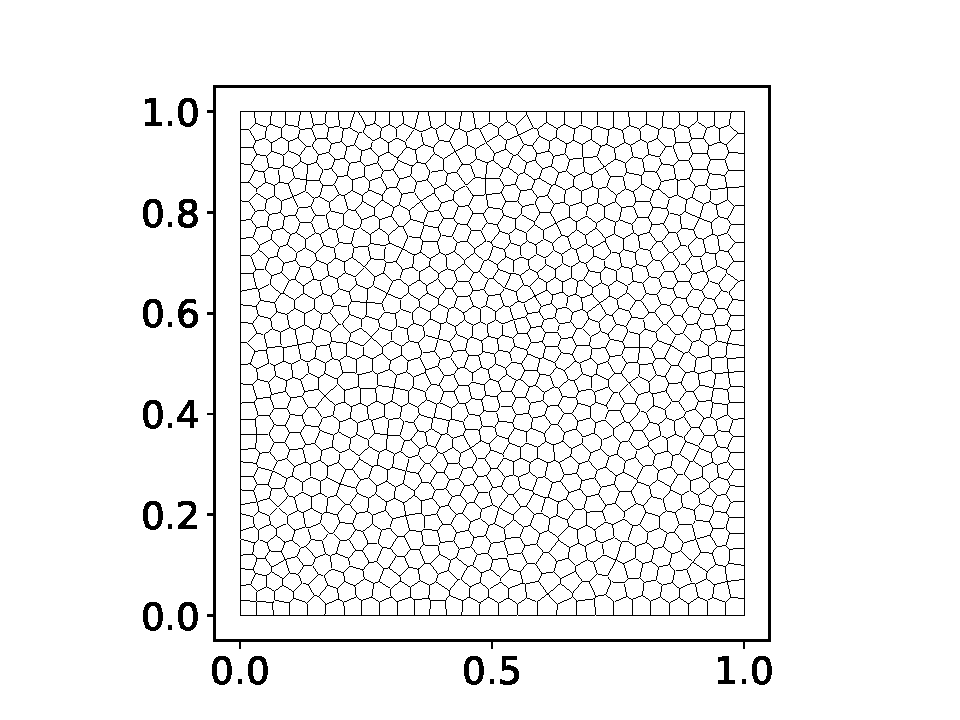
\includegraphics[trim=2cm 0.5cm 2cm 0.5cm, clip, width=0.45\textwidth]{meshes/uniform/square_1000.pdf}
        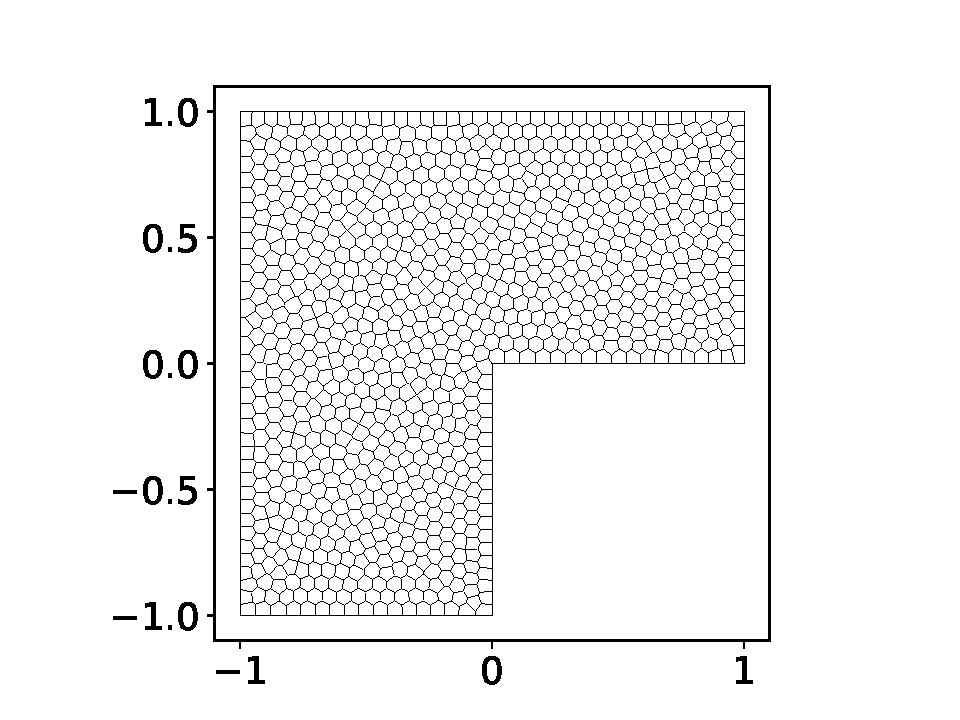
\includegraphics[trim=2cm 0.5cm 2cm 0.5cm, clip, width=0.45\textwidth]{meshes/uniform/lshape_1000.pdf}
        \caption{Square and L-shaped meshes over polygonal domains with $N = 1000$ elements.}
    \end{figure}
\end{frame}

\begin{frame}
    \frametitle{Mesh-building strategy}

    The mesh-building strategy involves the following steps:

    \begin{enumerate}
        \item Generate a Voronoi diagram to partition the domain into regions based on point locations.
        \item Refine the mesh by adjusting point positions to minimize element distortion.
        \item Remove or adjust very small edges to enhance mesh quality and stability.
        \item Analyze the connectivity and arrangement of mesh elements to ensure proper structure.
        \item Calculate properties such as element areas and the largest simplices.
    \end{enumerate}

\end{frame}

\begin{frame}[fragile]
    \frametitle{\lstinline{mesh_diagram}}

    Most steps of the mesh-building process are carried out by \lstinline{mesh_diagram}.

    \begin{lstlisting}[style=cpp]
    std::vector<Polygon> mesh_diagram(
        const Polygon &, 
        const std::size_t &, 
        const bool &reflect = false, 
        const bool &uniform = false
    );
    \end{lstlisting}

\end{frame}